\begin{figure}[H]
  \centering
  \begin{subfigure}[t]{.48\linewidth}
    \centering
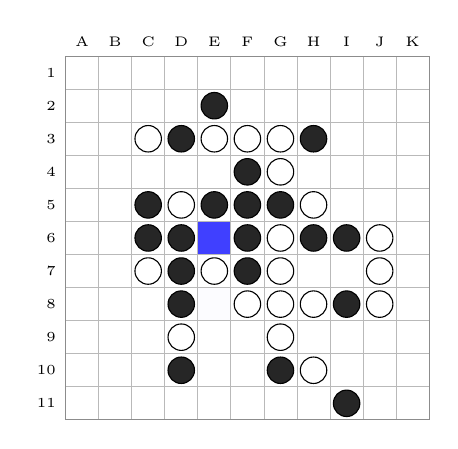
\begin{tikzpicture}[x=0.42cm, y=0.42cm]
\fill[blue!75] (4,-5) rectangle (5,-6);
\fill[blue!1] (4,-7) rectangle (5,-8);
\draw[gray!55, line width=.3pt, step=1] (0,0) grid (11,-11);
\draw[gray!90] (0,0) rectangle (11,-11);
\node[font=\tiny, anchor=south] at (0.5,0) {A};
\node[font=\tiny, anchor=south] at (1.5,0) {B};
\node[font=\tiny, anchor=south] at (2.5,0) {C};
\node[font=\tiny, anchor=south] at (3.5,0) {D};
\node[font=\tiny, anchor=south] at (4.5,0) {E};
\node[font=\tiny, anchor=south] at (5.5,0) {F};
\node[font=\tiny, anchor=south] at (6.5,0) {G};
\node[font=\tiny, anchor=south] at (7.5,0) {H};
\node[font=\tiny, anchor=south] at (8.5,0) {I};
\node[font=\tiny, anchor=south] at (9.5,0) {J};
\node[font=\tiny, anchor=south] at (10.5,0) {K};
\node[font=\tiny, anchor=east] at (0,-0.5) {1};
\node[font=\tiny, anchor=east] at (0,-1.5) {2};
\node[font=\tiny, anchor=east] at (0,-2.5) {3};
\node[font=\tiny, anchor=east] at (0,-3.5) {4};
\node[font=\tiny, anchor=east] at (0,-4.5) {5};
\node[font=\tiny, anchor=east] at (0,-5.5) {6};
\node[font=\tiny, anchor=east] at (0,-6.5) {7};
\node[font=\tiny, anchor=east] at (0,-7.5) {8};
\node[font=\tiny, anchor=east] at (0,-8.5) {9};
\node[font=\tiny, anchor=east] at (0,-9.5) {10};
\node[font=\tiny, anchor=east] at (0,-10.5) {11};
\draw[fill=black!85, line width=.4pt] (4.5,-1.5) circle (.40);
\draw[fill=white, line width=.4pt] (2.5,-2.5) circle (.40);
\draw[fill=black!85, line width=.4pt] (3.5,-2.5) circle (.40);
\draw[fill=white, line width=.4pt] (4.5,-2.5) circle (.40);
\draw[fill=white, line width=.4pt] (5.5,-2.5) circle (.40);
\draw[fill=white, line width=.4pt] (6.5,-2.5) circle (.40);
\draw[fill=black!85, line width=.4pt] (7.5,-2.5) circle (.40);
\draw[fill=black!85, line width=.4pt] (5.5,-3.5) circle (.40);
\draw[fill=white, line width=.4pt] (6.5,-3.5) circle (.40);
\draw[fill=black!85, line width=.4pt] (2.5,-4.5) circle (.40);
\draw[fill=white, line width=.4pt] (3.5,-4.5) circle (.40);
\draw[fill=black!85, line width=.4pt] (4.5,-4.5) circle (.40);
\draw[fill=black!85, line width=.4pt] (5.5,-4.5) circle (.40);
\draw[fill=black!85, line width=.4pt] (6.5,-4.5) circle (.40);
\draw[fill=white, line width=.4pt] (7.5,-4.5) circle (.40);
\draw[fill=black!85, line width=.4pt] (2.5,-5.5) circle (.40);
\draw[fill=black!85, line width=.4pt] (3.5,-5.5) circle (.40);
\draw[fill=black!85, line width=.4pt] (5.5,-5.5) circle (.40);
\draw[fill=white, line width=.4pt] (6.5,-5.5) circle (.40);
\draw[fill=black!85, line width=.4pt] (7.5,-5.5) circle (.40);
\draw[fill=black!85, line width=.4pt] (8.5,-5.5) circle (.40);
\draw[fill=white, line width=.4pt] (9.5,-5.5) circle (.40);
\draw[fill=white, line width=.4pt] (2.5,-6.5) circle (.40);
\draw[fill=black!85, line width=.4pt] (3.5,-6.5) circle (.40);
\draw[fill=white, line width=.4pt] (4.5,-6.5) circle (.40);
\draw[fill=black!85, line width=.4pt] (5.5,-6.5) circle (.40);
\draw[fill=white, line width=.4pt] (6.5,-6.5) circle (.40);
\draw[fill=white, line width=.4pt] (9.5,-6.5) circle (.40);
\draw[fill=black!85, line width=.4pt] (3.5,-7.5) circle (.40);
\draw[fill=white, line width=.4pt] (5.5,-7.5) circle (.40);
\draw[fill=white, line width=.4pt] (6.5,-7.5) circle (.40);
\draw[fill=white, line width=.4pt] (7.5,-7.5) circle (.40);
\draw[fill=black!85, line width=.4pt] (8.5,-7.5) circle (.40);
\draw[fill=white, line width=.4pt] (9.5,-7.5) circle (.40);
\draw[fill=white, line width=.4pt] (3.5,-8.5) circle (.40);
\draw[fill=white, line width=.4pt] (6.5,-8.5) circle (.40);
\draw[fill=black!85, line width=.4pt] (3.5,-9.5) circle (.40);
\draw[fill=black!85, line width=.4pt] (6.5,-9.5) circle (.40);
\draw[fill=white, line width=.4pt] (7.5,-9.5) circle (.40);
\draw[fill=black!85, line width=.4pt] (8.5,-10.5) circle (.40);
\end{tikzpicture}
    \caption{SL v3: $v=0{,}89$; đáp án 99,7\%; cao nhất E6 (97,7\%)}
  \end{subfigure}\hfill
  \begin{subfigure}[t]{.48\linewidth}
    \centering
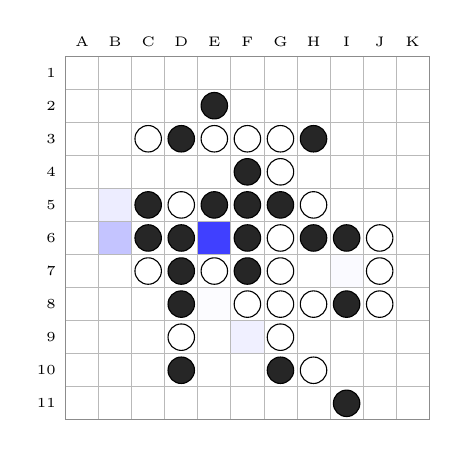
\begin{tikzpicture}[x=0.42cm, y=0.42cm]
\fill[blue!7] (1,-4) rectangle (2,-5);
\fill[blue!23] (1,-5) rectangle (2,-6);
\fill[blue!75] (4,-5) rectangle (5,-6);
\fill[blue!2] (8,-6) rectangle (9,-7);
\fill[blue!1] (4,-7) rectangle (5,-8);
\fill[blue!6] (5,-8) rectangle (6,-9);
\draw[gray!55, line width=.3pt, step=1] (0,0) grid (11,-11);
\draw[gray!90] (0,0) rectangle (11,-11);
\node[font=\tiny, anchor=south] at (0.5,0) {A};
\node[font=\tiny, anchor=south] at (1.5,0) {B};
\node[font=\tiny, anchor=south] at (2.5,0) {C};
\node[font=\tiny, anchor=south] at (3.5,0) {D};
\node[font=\tiny, anchor=south] at (4.5,0) {E};
\node[font=\tiny, anchor=south] at (5.5,0) {F};
\node[font=\tiny, anchor=south] at (6.5,0) {G};
\node[font=\tiny, anchor=south] at (7.5,0) {H};
\node[font=\tiny, anchor=south] at (8.5,0) {I};
\node[font=\tiny, anchor=south] at (9.5,0) {J};
\node[font=\tiny, anchor=south] at (10.5,0) {K};
\node[font=\tiny, anchor=east] at (0,-0.5) {1};
\node[font=\tiny, anchor=east] at (0,-1.5) {2};
\node[font=\tiny, anchor=east] at (0,-2.5) {3};
\node[font=\tiny, anchor=east] at (0,-3.5) {4};
\node[font=\tiny, anchor=east] at (0,-4.5) {5};
\node[font=\tiny, anchor=east] at (0,-5.5) {6};
\node[font=\tiny, anchor=east] at (0,-6.5) {7};
\node[font=\tiny, anchor=east] at (0,-7.5) {8};
\node[font=\tiny, anchor=east] at (0,-8.5) {9};
\node[font=\tiny, anchor=east] at (0,-9.5) {10};
\node[font=\tiny, anchor=east] at (0,-10.5) {11};
\draw[fill=black!85, line width=.4pt] (4.5,-1.5) circle (.40);
\draw[fill=white, line width=.4pt] (2.5,-2.5) circle (.40);
\draw[fill=black!85, line width=.4pt] (3.5,-2.5) circle (.40);
\draw[fill=white, line width=.4pt] (4.5,-2.5) circle (.40);
\draw[fill=white, line width=.4pt] (5.5,-2.5) circle (.40);
\draw[fill=white, line width=.4pt] (6.5,-2.5) circle (.40);
\draw[fill=black!85, line width=.4pt] (7.5,-2.5) circle (.40);
\draw[fill=black!85, line width=.4pt] (5.5,-3.5) circle (.40);
\draw[fill=white, line width=.4pt] (6.5,-3.5) circle (.40);
\draw[fill=black!85, line width=.4pt] (2.5,-4.5) circle (.40);
\draw[fill=white, line width=.4pt] (3.5,-4.5) circle (.40);
\draw[fill=black!85, line width=.4pt] (4.5,-4.5) circle (.40);
\draw[fill=black!85, line width=.4pt] (5.5,-4.5) circle (.40);
\draw[fill=black!85, line width=.4pt] (6.5,-4.5) circle (.40);
\draw[fill=white, line width=.4pt] (7.5,-4.5) circle (.40);
\draw[fill=black!85, line width=.4pt] (2.5,-5.5) circle (.40);
\draw[fill=black!85, line width=.4pt] (3.5,-5.5) circle (.40);
\draw[fill=black!85, line width=.4pt] (5.5,-5.5) circle (.40);
\draw[fill=white, line width=.4pt] (6.5,-5.5) circle (.40);
\draw[fill=black!85, line width=.4pt] (7.5,-5.5) circle (.40);
\draw[fill=black!85, line width=.4pt] (8.5,-5.5) circle (.40);
\draw[fill=white, line width=.4pt] (9.5,-5.5) circle (.40);
\draw[fill=white, line width=.4pt] (2.5,-6.5) circle (.40);
\draw[fill=black!85, line width=.4pt] (3.5,-6.5) circle (.40);
\draw[fill=white, line width=.4pt] (4.5,-6.5) circle (.40);
\draw[fill=black!85, line width=.4pt] (5.5,-6.5) circle (.40);
\draw[fill=white, line width=.4pt] (6.5,-6.5) circle (.40);
\draw[fill=white, line width=.4pt] (9.5,-6.5) circle (.40);
\draw[fill=black!85, line width=.4pt] (3.5,-7.5) circle (.40);
\draw[fill=white, line width=.4pt] (5.5,-7.5) circle (.40);
\draw[fill=white, line width=.4pt] (6.5,-7.5) circle (.40);
\draw[fill=white, line width=.4pt] (7.5,-7.5) circle (.40);
\draw[fill=black!85, line width=.4pt] (8.5,-7.5) circle (.40);
\draw[fill=white, line width=.4pt] (9.5,-7.5) circle (.40);
\draw[fill=white, line width=.4pt] (3.5,-8.5) circle (.40);
\draw[fill=white, line width=.4pt] (6.5,-8.5) circle (.40);
\draw[fill=black!85, line width=.4pt] (3.5,-9.5) circle (.40);
\draw[fill=black!85, line width=.4pt] (6.5,-9.5) circle (.40);
\draw[fill=white, line width=.4pt] (7.5,-9.5) circle (.40);
\draw[fill=black!85, line width=.4pt] (8.5,-10.5) circle (.40);
\end{tikzpicture}
    \caption{SL không aug: $v=0{,}60$; đáp án 86,8\%; cao nhất E6 (66,3\%)}
  \end{subfigure}\par\medskip
  \begin{subfigure}[t]{.48\linewidth}
    \centering
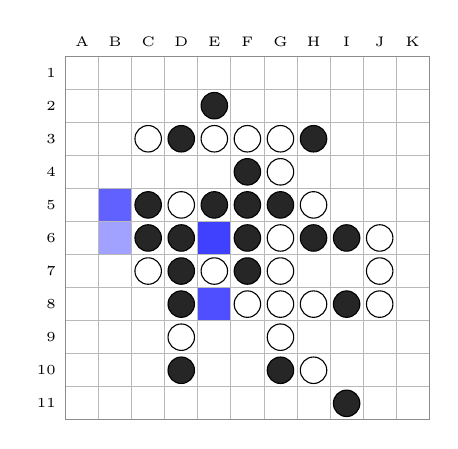
\begin{tikzpicture}[x=0.42cm, y=0.42cm]
\fill[blue!62] (1,-4) rectangle (2,-5);
\fill[blue!37] (1,-5) rectangle (2,-6);
\fill[blue!75] (4,-5) rectangle (5,-6);
\fill[blue!69] (4,-7) rectangle (5,-8);
\draw[gray!55, line width=.3pt, step=1] (0,0) grid (11,-11);
\draw[gray!90] (0,0) rectangle (11,-11);
\node[font=\tiny, anchor=south] at (0.5,0) {A};
\node[font=\tiny, anchor=south] at (1.5,0) {B};
\node[font=\tiny, anchor=south] at (2.5,0) {C};
\node[font=\tiny, anchor=south] at (3.5,0) {D};
\node[font=\tiny, anchor=south] at (4.5,0) {E};
\node[font=\tiny, anchor=south] at (5.5,0) {F};
\node[font=\tiny, anchor=south] at (6.5,0) {G};
\node[font=\tiny, anchor=south] at (7.5,0) {H};
\node[font=\tiny, anchor=south] at (8.5,0) {I};
\node[font=\tiny, anchor=south] at (9.5,0) {J};
\node[font=\tiny, anchor=south] at (10.5,0) {K};
\node[font=\tiny, anchor=east] at (0,-0.5) {1};
\node[font=\tiny, anchor=east] at (0,-1.5) {2};
\node[font=\tiny, anchor=east] at (0,-2.5) {3};
\node[font=\tiny, anchor=east] at (0,-3.5) {4};
\node[font=\tiny, anchor=east] at (0,-4.5) {5};
\node[font=\tiny, anchor=east] at (0,-5.5) {6};
\node[font=\tiny, anchor=east] at (0,-6.5) {7};
\node[font=\tiny, anchor=east] at (0,-7.5) {8};
\node[font=\tiny, anchor=east] at (0,-8.5) {9};
\node[font=\tiny, anchor=east] at (0,-9.5) {10};
\node[font=\tiny, anchor=east] at (0,-10.5) {11};
\draw[fill=black!85, line width=.4pt] (4.5,-1.5) circle (.40);
\draw[fill=white, line width=.4pt] (2.5,-2.5) circle (.40);
\draw[fill=black!85, line width=.4pt] (3.5,-2.5) circle (.40);
\draw[fill=white, line width=.4pt] (4.5,-2.5) circle (.40);
\draw[fill=white, line width=.4pt] (5.5,-2.5) circle (.40);
\draw[fill=white, line width=.4pt] (6.5,-2.5) circle (.40);
\draw[fill=black!85, line width=.4pt] (7.5,-2.5) circle (.40);
\draw[fill=black!85, line width=.4pt] (5.5,-3.5) circle (.40);
\draw[fill=white, line width=.4pt] (6.5,-3.5) circle (.40);
\draw[fill=black!85, line width=.4pt] (2.5,-4.5) circle (.40);
\draw[fill=white, line width=.4pt] (3.5,-4.5) circle (.40);
\draw[fill=black!85, line width=.4pt] (4.5,-4.5) circle (.40);
\draw[fill=black!85, line width=.4pt] (5.5,-4.5) circle (.40);
\draw[fill=black!85, line width=.4pt] (6.5,-4.5) circle (.40);
\draw[fill=white, line width=.4pt] (7.5,-4.5) circle (.40);
\draw[fill=black!85, line width=.4pt] (2.5,-5.5) circle (.40);
\draw[fill=black!85, line width=.4pt] (3.5,-5.5) circle (.40);
\draw[fill=black!85, line width=.4pt] (5.5,-5.5) circle (.40);
\draw[fill=white, line width=.4pt] (6.5,-5.5) circle (.40);
\draw[fill=black!85, line width=.4pt] (7.5,-5.5) circle (.40);
\draw[fill=black!85, line width=.4pt] (8.5,-5.5) circle (.40);
\draw[fill=white, line width=.4pt] (9.5,-5.5) circle (.40);
\draw[fill=white, line width=.4pt] (2.5,-6.5) circle (.40);
\draw[fill=black!85, line width=.4pt] (3.5,-6.5) circle (.40);
\draw[fill=white, line width=.4pt] (4.5,-6.5) circle (.40);
\draw[fill=black!85, line width=.4pt] (5.5,-6.5) circle (.40);
\draw[fill=white, line width=.4pt] (6.5,-6.5) circle (.40);
\draw[fill=white, line width=.4pt] (9.5,-6.5) circle (.40);
\draw[fill=black!85, line width=.4pt] (3.5,-7.5) circle (.40);
\draw[fill=white, line width=.4pt] (5.5,-7.5) circle (.40);
\draw[fill=white, line width=.4pt] (6.5,-7.5) circle (.40);
\draw[fill=white, line width=.4pt] (7.5,-7.5) circle (.40);
\draw[fill=black!85, line width=.4pt] (8.5,-7.5) circle (.40);
\draw[fill=white, line width=.4pt] (9.5,-7.5) circle (.40);
\draw[fill=white, line width=.4pt] (3.5,-8.5) circle (.40);
\draw[fill=white, line width=.4pt] (6.5,-8.5) circle (.40);
\draw[fill=black!85, line width=.4pt] (3.5,-9.5) circle (.40);
\draw[fill=black!85, line width=.4pt] (6.5,-9.5) circle (.40);
\draw[fill=white, line width=.4pt] (7.5,-9.5) circle (.40);
\draw[fill=black!85, line width=.4pt] (8.5,-10.5) circle (.40);
\end{tikzpicture}
    \caption{L6 (RL): $v=-0{,}30$; đáp án 73,9\%; cao nhất E6 (30,6\%)}
  \end{subfigure}\hfill
  \begin{subfigure}[t]{.48\linewidth}
    \centering
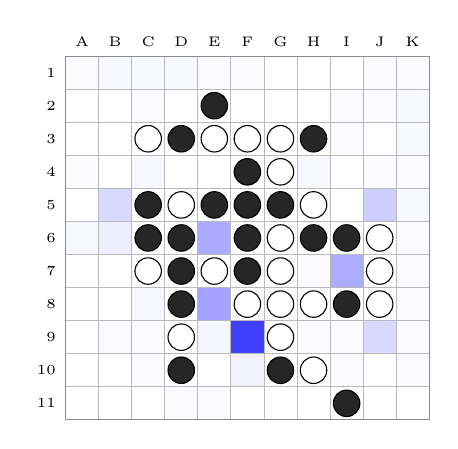
\begin{tikzpicture}[x=0.42cm, y=0.42cm]
\fill[blue!2] (0,0) rectangle (1,-1);
\fill[blue!3] (1,0) rectangle (2,-1);
\fill[blue!3] (2,0) rectangle (3,-1);
\fill[blue!3] (3,0) rectangle (4,-1);
\fill[blue!2] (4,0) rectangle (5,-1);
\fill[blue!2] (5,0) rectangle (6,-1);
\fill[blue!2] (9,0) rectangle (10,-1);
\fill[blue!2] (10,0) rectangle (11,-1);
\fill[blue!2] (2,-1) rectangle (3,-2);
\fill[blue!2] (8,-1) rectangle (9,-2);
\fill[blue!2] (9,-1) rectangle (10,-2);
\fill[blue!3] (10,-1) rectangle (11,-2);
\fill[blue!2] (8,-2) rectangle (9,-3);
\fill[blue!3] (10,-2) rectangle (11,-3);
\fill[blue!2] (0,-3) rectangle (1,-4);
\fill[blue!3] (2,-3) rectangle (3,-4);
\fill[blue!3] (7,-3) rectangle (8,-4);
\fill[blue!2] (9,-3) rectangle (10,-4);
\fill[blue!2] (10,-3) rectangle (11,-4);
\fill[blue!15] (1,-4) rectangle (2,-5);
\fill[blue!19] (9,-4) rectangle (10,-5);
\fill[blue!3] (10,-4) rectangle (11,-5);
\fill[blue!3] (0,-5) rectangle (1,-6);
\fill[blue!7] (1,-5) rectangle (2,-6);
\fill[blue!33] (4,-5) rectangle (5,-6);
\fill[blue!2] (10,-5) rectangle (11,-6);
\fill[blue!2] (7,-6) rectangle (8,-7);
\fill[blue!32] (8,-6) rectangle (9,-7);
\fill[blue!2] (10,-6) rectangle (11,-7);
\fill[blue!3] (2,-7) rectangle (3,-8);
\fill[blue!36] (4,-7) rectangle (5,-8);
\fill[blue!2] (10,-7) rectangle (11,-8);
\fill[blue!2] (1,-8) rectangle (2,-9);
\fill[blue!2] (2,-8) rectangle (3,-9);
\fill[blue!4] (4,-8) rectangle (5,-9);
\fill[blue!75] (5,-8) rectangle (6,-9);
\fill[blue!2] (7,-8) rectangle (8,-9);
\fill[blue!2] (8,-8) rectangle (9,-9);
\fill[blue!15] (9,-8) rectangle (10,-9);
\fill[blue!2] (10,-8) rectangle (11,-9);
\fill[blue!2] (2,-9) rectangle (3,-10);
\fill[blue!5] (5,-9) rectangle (6,-10);
\fill[blue!2] (8,-9) rectangle (9,-10);
\fill[blue!2] (10,-9) rectangle (11,-10);
\fill[blue!2] (3,-10) rectangle (4,-11);
\fill[blue!2] (4,-10) rectangle (5,-11);
\draw[gray!55, line width=.3pt, step=1] (0,0) grid (11,-11);
\draw[gray!90] (0,0) rectangle (11,-11);
\node[font=\tiny, anchor=south] at (0.5,0) {A};
\node[font=\tiny, anchor=south] at (1.5,0) {B};
\node[font=\tiny, anchor=south] at (2.5,0) {C};
\node[font=\tiny, anchor=south] at (3.5,0) {D};
\node[font=\tiny, anchor=south] at (4.5,0) {E};
\node[font=\tiny, anchor=south] at (5.5,0) {F};
\node[font=\tiny, anchor=south] at (6.5,0) {G};
\node[font=\tiny, anchor=south] at (7.5,0) {H};
\node[font=\tiny, anchor=south] at (8.5,0) {I};
\node[font=\tiny, anchor=south] at (9.5,0) {J};
\node[font=\tiny, anchor=south] at (10.5,0) {K};
\node[font=\tiny, anchor=east] at (0,-0.5) {1};
\node[font=\tiny, anchor=east] at (0,-1.5) {2};
\node[font=\tiny, anchor=east] at (0,-2.5) {3};
\node[font=\tiny, anchor=east] at (0,-3.5) {4};
\node[font=\tiny, anchor=east] at (0,-4.5) {5};
\node[font=\tiny, anchor=east] at (0,-5.5) {6};
\node[font=\tiny, anchor=east] at (0,-6.5) {7};
\node[font=\tiny, anchor=east] at (0,-7.5) {8};
\node[font=\tiny, anchor=east] at (0,-8.5) {9};
\node[font=\tiny, anchor=east] at (0,-9.5) {10};
\node[font=\tiny, anchor=east] at (0,-10.5) {11};
\draw[fill=black!85, line width=.4pt] (4.5,-1.5) circle (.40);
\draw[fill=white, line width=.4pt] (2.5,-2.5) circle (.40);
\draw[fill=black!85, line width=.4pt] (3.5,-2.5) circle (.40);
\draw[fill=white, line width=.4pt] (4.5,-2.5) circle (.40);
\draw[fill=white, line width=.4pt] (5.5,-2.5) circle (.40);
\draw[fill=white, line width=.4pt] (6.5,-2.5) circle (.40);
\draw[fill=black!85, line width=.4pt] (7.5,-2.5) circle (.40);
\draw[fill=black!85, line width=.4pt] (5.5,-3.5) circle (.40);
\draw[fill=white, line width=.4pt] (6.5,-3.5) circle (.40);
\draw[fill=black!85, line width=.4pt] (2.5,-4.5) circle (.40);
\draw[fill=white, line width=.4pt] (3.5,-4.5) circle (.40);
\draw[fill=black!85, line width=.4pt] (4.5,-4.5) circle (.40);
\draw[fill=black!85, line width=.4pt] (5.5,-4.5) circle (.40);
\draw[fill=black!85, line width=.4pt] (6.5,-4.5) circle (.40);
\draw[fill=white, line width=.4pt] (7.5,-4.5) circle (.40);
\draw[fill=black!85, line width=.4pt] (2.5,-5.5) circle (.40);
\draw[fill=black!85, line width=.4pt] (3.5,-5.5) circle (.40);
\draw[fill=black!85, line width=.4pt] (5.5,-5.5) circle (.40);
\draw[fill=white, line width=.4pt] (6.5,-5.5) circle (.40);
\draw[fill=black!85, line width=.4pt] (7.5,-5.5) circle (.40);
\draw[fill=black!85, line width=.4pt] (8.5,-5.5) circle (.40);
\draw[fill=white, line width=.4pt] (9.5,-5.5) circle (.40);
\draw[fill=white, line width=.4pt] (2.5,-6.5) circle (.40);
\draw[fill=black!85, line width=.4pt] (3.5,-6.5) circle (.40);
\draw[fill=white, line width=.4pt] (4.5,-6.5) circle (.40);
\draw[fill=black!85, line width=.4pt] (5.5,-6.5) circle (.40);
\draw[fill=white, line width=.4pt] (6.5,-6.5) circle (.40);
\draw[fill=white, line width=.4pt] (9.5,-6.5) circle (.40);
\draw[fill=black!85, line width=.4pt] (3.5,-7.5) circle (.40);
\draw[fill=white, line width=.4pt] (5.5,-7.5) circle (.40);
\draw[fill=white, line width=.4pt] (6.5,-7.5) circle (.40);
\draw[fill=white, line width=.4pt] (7.5,-7.5) circle (.40);
\draw[fill=black!85, line width=.4pt] (8.5,-7.5) circle (.40);
\draw[fill=white, line width=.4pt] (9.5,-7.5) circle (.40);
\draw[fill=white, line width=.4pt] (3.5,-8.5) circle (.40);
\draw[fill=white, line width=.4pt] (6.5,-8.5) circle (.40);
\draw[fill=black!85, line width=.4pt] (3.5,-9.5) circle (.40);
\draw[fill=black!85, line width=.4pt] (6.5,-9.5) circle (.40);
\draw[fill=white, line width=.4pt] (7.5,-9.5) circle (.40);
\draw[fill=black!85, line width=.4pt] (8.5,-10.5) circle (.40);
\end{tikzpicture}
    \caption{L8 (AZ): $v=-0{,}73$; đáp án 20,0\%; cao nhất F9 (19,9\%)}
  \end{subfigure}\par\medskip
  \caption{Policy của bốn mạng tại thế C4-001 (X đi). Ô càng đậm xác suất càng cao (chuẩn hoá theo ô lớn nhất của từng mạng). Đáp án: B6, E6, E8.}
  \label{fig:cs-policy-c4}
\end{figure}
